\documentclass[10pt]{article}
\usepackage[a4paper,margin=20mm]{geometry}
\usepackage{amsmath,amssymb,graphicx,booktabs}
\newcommand{\TODO}[1]{\textbf{[#1]}}
\begin{document}
\newcommand{\eqrefx}[1]{(#1)}
\makeatletter
\providecommand{\eqoffsetbound}{}
\makeatother
\def\eqoffsetbound{}
% ---------------------------------------------------------------------
% Drop-in for the RESULTS section: the a priori bound of Sec. VI-E
% checked against the campaign.
%
% Place after the offset results and before the realised budget.  The
% float is a two-column figure*; the file is docs/fig_bound_validation.pdf,
% regenerated by
%     python analysis/error_budget.py DataSet/exp --output-dir docs
%     python analysis/bound_validation_figure.py docs docs/fig_bound_validation.pdf
%
% Numbering: (109) is the boxed bound of Sec. VI-E, (107) its weight,
% (90) the rate-deviation bound.  Renumber if the host differs.
%
% NOTE the check is deliberately forward.  It is tempting to compare the
% bound against the prediction residual instead, and that comparison is
% ill-posed rather than merely loose: the onset is chosen to minimise the
% residual, so the component of the deviation the bound is about is
% removed from the residual by identity.  The paragraph below says so
% once, briefly, because a reader who tries it will otherwise conclude
% the bound fails.
% ---------------------------------------------------------------------

\begin{figure*}[t]
\centering
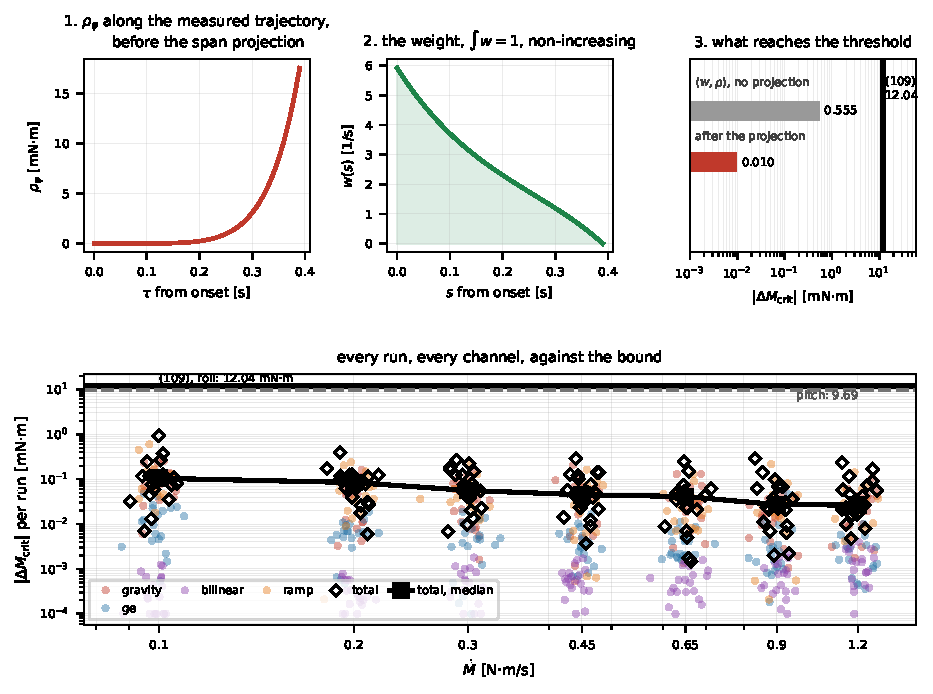
\includegraphics[width=\linewidth]{fig_bound_validation.pdf}
\caption{The a priori bound (109) checked forwards on
the campaign. \emph{Top, one run} (case~1, roll, $\dot M = 1.20$~N\,m/s):
the gravity remainder $\rho_\varphi$ evaluated along the measured
trajectory; the normalised weight $w$ of (107), which
integrates to one and decreases, so that the forcing is largest exactly
where the weight is least; and the resulting displacement, before and
after the estimator's own degrees of freedom are projected out, against
the bound. \emph{Bottom, all $140$ runs}: the displacement per run and
per channel. Every run lies inside, by a factor of $246$ in the median
and $13$ at worst, and the gravity channel dominates as the bound
predicts. The fit residual enters this chain nowhere; see the text.}

\end{figure*}

\subsection{The a priori bound against the campaign}


Sec.~VI-E bounds the displacement of the identified threshold
by the two forcing terms the estimator cannot absorb, giving
$0.400$~mm of equivalent offset for roll and $0.322$ for pitch over the
admissible box. That bound is made before the campaign, from a scale,
a CAD inertia and the excitation protocol; what remains is to ask what
the runs actually do.

The question has to be put forwards. Each perturbation is evaluated
along the \emph{measured} trajectory over the fit window, projected out
of the estimator's own per-run degrees of freedom $\{1,\tau,
\delta\varphi\}$, propagated through the Duhamel integral of the
deviation dynamics, and correlated against the weight of
(107). Fig.~\ref{fig:bound-validation} shows that chain on
one run and its result on all of them. The displacement is $0.049$~mN\,m
in the median, $0.161$ at p90 and $0.927$ at worst, against the
$12.04$~mN\,m the bound allows: every one of the $140$ runs is inside,
with two orders of margin typically and a factor of $13$ in the worst
case. The split across channels is the one the bound assumes, the
gravity remainder supplying almost all of it and the ground-effect
coupling two decades less.

Two features of the chain are worth reading off the top row. The
forcing rises steeply towards the end of the window, as
$\rho_\varphi\propto\varphi^2$ must, while the weight falls
monotonically from the onset --- the pairing that Chebyshev's inequality
turns into the factors $\tfrac17$ and $\tfrac15$, and the reason the
bound is four times sharper than the envelope it replaces. And the
projection is not a detail: on the run shown it takes the displacement
from $0.555$ to $0.010$~mN\,m, the estimator absorbing what looks to it
like a shifted onset.

\paragraph{Why the prediction residual is not this check.}
It is natural to compare the bound with the residual of
Sec.~VI-A instead, and the comparison is ill-posed rather
than merely conservative. The bound is on the deviation from the
nominal response at the true onset; the residual is the deviation from
a curve whose onset was chosen so as to minimise that residual.
Whatever part of the deviation lies along $\partial\hat\omega/\partial
t_c\propto\sinh C_2\tau$ is therefore removed by identity, so the
residual is everything orthogonal to the estimator's span while the
displacement bounded here is exactly the projection the residual
discards. The two partition the deviation between them and neither
carries information about the other. Pointwise the mismatch is
conspicuous --- the bound's envelope leaves the onset like $\tau^7$
while the measurement starts at the gyro noise floor, so the residual
sits outside it over $90\%$ of the window at every ramp rate --- and
none of that bears on the bound. The residual is a prediction test on
the model shape, reported as such in Sec.~VI-A; the
bound is checked here, forwards.
\end{document}
